\documentclass[a4paper, 12pt]{article}
\usepackage{geometry}
\geometry{a4paper,
total={170mm,257mm},left=2cm,right=2cm,
top=2cm,bottom=2cm}

\usepackage{mathtext}
\usepackage{amsmath}
\usepackage[T2A]{fontenc}
\usepackage[utf8]{inputenc}
\usepackage[english,russian]{babel}
\usepackage{graphicx, float}
\usepackage{tabularx, colortbl}
\usepackage{caption}
\captionsetup{labelsep=period}

\newcommand{\parag}[1]{\paragraph*{#1:}}
\DeclareSymbolFont{T2Aletters}{T2A}{cmr}{m}{it}
\newcounter{Points}
\setcounter{Points}{1}
\newcommand{\point}{\arabic{Points}. \addtocounter{Points}{1}}
\newcolumntype{C}{>{\centering\arraybackslash}X}

\author{Калинин Даниил, Б01-110}
\date{\today}
\title{Лабораторная работа 2.2.1. Исследование взаимной диффузии газов}

\begin{document}
\maketitle

\parag {Цель работы}

\begin{enumerate}
	\item регистрация зависимости концентрации гелия в воздухе от времени с помощью датчиков теплопроводности при разных начальных давлениях смеси газов;
	\item определение коэффициента диффузии по результатам измерений.
\end{enumerate}

\parag {В работе используются}
измерительная установка; форвакуумный насос; баллон с газом (гелий); манометр; источник питания; магазин сопротивлений; гальванометр; секундомер.

\parag {Теоритическая справка} ~\\
Диффузией называют самопроизвольное взаимное проникновение веществ друг в друга, происходящее вследствие хаотичного теплового движения молекул. При перемешивании молекул разного сорта говорят о взаимной (или концентрационной) диффузии.

Диффузия в системе, состоящей из двух компонентов $ a $ и $ b $ (бинарная смесь), подчиняется закону Фика: плотности потока компонентов $ j_{a,b} $ (количество частиц, пересекающих единичную площадку в единицу времени) пропорциональны градиентам их концентраций $ \nabla n_{a,b}$, что в одномерном случае можно записать как

\[ j_a = -D\frac{\partial n_a}{\partial x}, \quad j_b = -D\frac{\partial n_b}{\partial x}, \]
где $ D $ -- коэффициент взаимной диффузии компонентов. Знак <<минус>> отражает тот факт, что диффузия идёт в направлении выравнивания концентраций. Равновесие достигается при равномерном распределении вещества по объёму сосуда ($ \partial n / \partial x = 0 $).

В данной работе исследуется взаимная диффузия гелия и воздуха. Давление P и температура T в условиях опыта предполагаются неизменными: $ p=(n_{He}+n_{\text{в}})kT $, где $ n_{He} $ и $ n_{\text{в}} $ -- концентрации (объёмные плотности) диффундирующих газов. Поэтому для любых изменений концентраций справедливо $ \Delta n_{He}=-\Delta n_{\text{в}} $. Следовательно, достаточно ограничиться описанием диффузии одного из компонентов, например гелия $ n_{He} $:

\begin{equation}\label{1}
j_{He}=-D\frac{\partial n_{He}}{\partial x}.
\end{equation}

Приведём теоретическую оценку для коэффициента диффузии. В работе концентрация гелия, как правило, мала $ (n_{He} \ll n_\text{в}) $. Кроме того, атомы гелия существенно легче молекул, составляющих воздух ($ \mu_{He} \ll \mu_{O_2}, \mu_{N_2} $), значит и их средняя тепловая скорость велика по сравнению с остальными частицами. Поэтому перемешивание газов в работе можно приближенно описывать как диффузию примеси лёгких частиц $ He $ на практически стационарном фоне воздуха. Коэффициент диффузии в таком приближении равен

\begin{equation}\label{2}
D=\frac{1}{3}\lambda \overline{v},
\end{equation}

где $ \overline{v}=\sqrt{\frac{8RT}{\pi \mu}} $ -- средняя тепловая скорость частиц примеси, $ \lambda = \frac{1}{n_0\sigma} $ -- их длина свободного пробега, $ n_0 $ -- концентрация рассеивающих центров (фона), $ \sigma $ -- сечение столкновения частиц примеси с частицами фона.

Таким образом, теория предсказывает, что коэффициент диффузии бинарной смеси обратно пропорционален давлению в системе $ D \propto 1/P $, и не зависит от пропорций компонентов, что и предлагается проверить в работе экспериментально.

\parag {Схема эксперимента}~\\

Для исследования взаимной диффузии газов и измерения коэффициента взаимной диффузии $ D $ используется два сосуда объёмами $ V_1 $ и $ V_2 $ $ (V_1\approx V_2=V) $, соединенные трубкой длины $ L $ и сечения $ S $. Предполагается, что сосуды заполнены смесью двух газов при одинаковом давлении, но с различной концентрацией компонентов. Вследствие взаимной диффузии, проходящей в соединительной трубке, концентрации компонентов в сосудах с течением времени выравниваются. 

В общем случае концентрации компонентов $ n(t, x) $ зависят от как от координаты, так и времени. Задача упрощается, если объём соединительной трубки мал по сравнению с объёмами сосудов -- тогда концентрации газов $ n_1(t) $ и $ n_2(t) $ внутри каждого сосуда можно считать постоянными по всему объёму сосуда, и принять, что процесс выравнивания концентраций происходит благодаря диффузии в трубке.

Рассмотрим подзадачу о диффузии в соединительной трубке. Предположим сперва, что концентрации примеси (гелия) на её торцах поддерживаются постоянными и равными $ n_1 $ и $ n_2 $ соответственно. Тогда через некоторое время в трубке установится стационарный поток частиц, одинаковый в каждом сечении трубки (в противном случае, если бы поток зависел от $ x $, частицы бы накапливались в трубке, и процесс перестал бы быть стационарным). Применяя закон Фика в трубке, получим

\[ j=-D\frac{\partial n}{\partial x} = const \]

Следовательно, распределение концентрации в трубке $ n(x) $ -- линейная
функция:

\begin{equation}\label{3}
n(x) = \frac{\Delta n}{L} x
\end{equation}
и плотность потока частиц всюду постоянна и равна

\begin{equation}\label{4}
j=-D\frac{\Delta n}{L},
\end{equation}
где $ \Delta n = n_2-n_1 $ -- разность концентраций гелия на концах трубки.

Теперь вернёмся к процессу выравнивания концентраций в сосудах. Частицы перетекают из сосуда 2 в сосуд 1 по трубке и концентрации $ n_1(t) $ и $ n_2(t) $ меняются во времени. Предположим, что этот процесс происходит достаточно медленно, так что в трубке в любой момент времени успевает установиться практически стационарное течение, описываемое формулами \eqref{3}, \eqref{4}. Такое приближение называют квазистационарным. Кроме того, будем считать, что в пределах каждого сосуда частицы распределены равномерно, так что концентрации примеси вблизи трубки и в остальных частях сосуда отличаются мало. Тогда полное число частиц примеси в сосудах равно соответственно $ N_1=n_1V $ и $ N_2=n_2V $. Произведение плотности потока \eqref{4} на площадь сечения трубки $ S $ даёт количество частиц, пересекающих в единицу времени любое поперечное сечение трубки. Поэтому

\begin{equation}\label{5}
    \frac{dN_1}{dt}=jS, \quad \frac{dN_2}{dt}=-jS.
\end{equation}

Выразим отсюда скорость изменения $ \Delta n $. Вычитая из второго равенства первое и деля результат на объём сосуда $ V $, с учетом \eqref{4} получим

\begin{equation}\label{6}
    \frac{d(\Delta n)}{dt}=-\frac{\Delta n}{\tau},
\end{equation}
где введено обозначение

\begin{equation}\label{7}
    \tau=\frac{1}{D}\frac{VL}{2S}.
\end{equation}

Интегрируя \eqref{6}, получаем, что разность концентраций будет убывать по экспоненциальному закону

\begin{equation}\label{8}
    \Delta n = \Delta n_0 e^{-t/\tau},
\end{equation}
где $ \Delta n_0 $ -- разность концентраций примеси в сосудах в начальный момент времени. Видно, что величина $ \tau $ есть характерное время выравнивания концентраций между сосудами. Оно определяется геометрическими размерами установки и коэффициентом диффузии.\\

\parag {Метод измерения}~\\

Для измерения разности концентраций в установке применяются датчики теплопроводности. При этом используется тот факт, что теплопроводность $ \kappa $ смеси зависит от её состава. В общем случае зависимость $ \kappa(n) $ довольно сложна, однако при малой разности $ \Delta n $ концентраций в сосудах можно ожидать, что разность теплопроводностей будет изменяться прямо пропорционально $ \Delta n $:

\[ \Delta \kappa = \kappa(n_2)-\kappa(n_1)\approx\text{const}\cdot\Delta n. \]

Эксперименты показывают, что если доля примеси гелия составляет менее
15\%, отклонение от линейной зависимости не превышает 0,5\%, что для наших целей вполне достаточно.

Сами датчики теплопроводности устроены следующим образом. Тонкая платиновая проволочка, протянутая вдоль оси стеклянного цилиндра, нагревается током. При заданной мощности нагревания, приращение температуры проволочки и, следовательно, приращение её сопротивления пропорциональны теплопроводности газа.

Для измерения сопротивлений используется мостовая схема, позволяющая определять разность показаний датчиков с высокой точностью. Мост балансируется при заполнении сосудов (и датчиков) одной и той же смесью. При заполнении сосудов смесями различного состава возникает разбаланc моста. При незначительном различии в составах смесей показания вольтметра, подсоединённого к диагонали моста, будут пропорциональны разности концентраций примеси: $ U\propto\Delta\kappa\propto\Delta n $. В процессе диффузии разность концентраций убывает по закону \eqref{8}, и значит по тому же закону изменяется напряжение:

\begin{equation}
    \label{10}
    U=U_0e^{-t/\tau},
\end{equation}
где $ U_0 $ -- показание гальванометра в начальный момент времени. Измеряя экспериментально зависимость $ U(t) $, можно получить характерное время
процесса $ \tau $, откуда по формуле \eqref{7} определить коэффициент диффузии $ D $.
    

\parag {Экспериментальная установка}~\\
В работе использовалось несколько типов установок, отличающихся схемами подачи газов. Схема установки, использовавшейся в данной работе приведена на рис. \ref{setup}. Измерительная часть соединена с системой откачки и напуска воздуха и гелия. Для откачки используется форвакуумный насос.

В данной работе использовалась компьютеризированная установка, которая позволяет записывать зависимость показаний вольтметра $ U(t) $ в реальном времени.

\begin{figure}
    \centering
	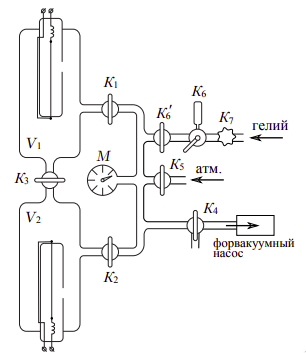
\includegraphics[width=8cm]{setup.png}
	\caption{Схема установки}
	\label{setup}
\end{figure}

\parag {Ход работы} ~\\
\point Запишем инструментальные погрешности измерений.

\begin{itemize}
    \item манометр -- 0,5 $кгс/см^2$
    \item вольтметр -- 0.1 мВ
    \item обьем -- $10 \ см^3$
\end{itemize}

\point Измерение коэффициента взаимной диффузии в зависимости от давления
Для смеси гелий-воздух исследуем зависимость коэффициента взаимной диффузии от начального давления. С помощью компьютера будем фиксировать изменение показаний вольтметра от прошедшего времени. По полученным данным построим график зависимости напряжения от времени в логарифмическом масштабе по оси ординат. График изображен на рисунке \ref{u_from_t_graph}

\begin{figure}
    \centering
	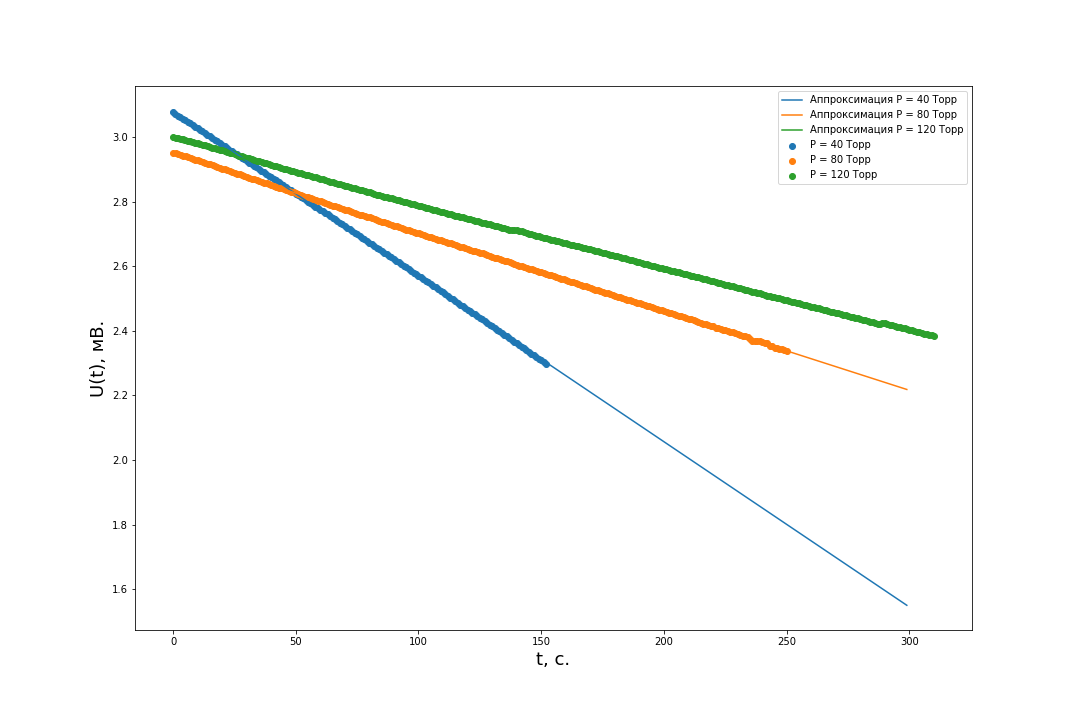
\includegraphics[width=\linewidth]{U_from_t_graph.png}
	\caption{График зависимости напряжения от времени}
	\label{u_from_t_graph}
\end{figure}

Из графика видно, что в логарифмическом масштабе зависимости принимают линейный вид. Поэтому проведём их аппроксимацию прямыми вида \[ y=Ae^{Bx}. \] Это уравнение при помощи логарифмирования можно привести к виду \[ \ln y = \ln A + Bx. \] Тогда в этом случаем для вычисления параметра $ B $ можно воспользоваться методом наименьших квадратов. Получаем следующее:

\begin{equation}\label{mnk:B}
B=\frac{\langle t\ln U \rangle - \langle t\rangle \langle \ln U\rangle}{\langle t^2 \rangle - \langle t \rangle^2}
\end{equation}

\begin{equation}\label{mnk:sigmaB}
\sigma^\text{случ}_B = \sqrt{\frac{1}{N-2} \left(\frac{\left\langle\left(\ln U - \langle \ln U\right\rangle\right)^2 \rangle}{\left\langle\left(t - \langle t\right\rangle\right)^2 \rangle}\right)-B^2},
\end{equation}
где N -- колличество измерений. При этом можно считать, что $ \sigma_B \approx \sigma_B^\text{случ} $, т.к. показания вольтметра довольно точны и систематическая ошибка мала по сравнению со случайными флуктуациями напряжения в ходе эксперимента.


Проводя данные вычисления для каждого значения, заносим результаты в таблицу \ref{tab:approx}.

\begin{table}
	\centering
	\begin{tabular}{|c|c|c|c|c|}
		\hline
		$ P $, торр & $ B \cdot 10^{-3} $, с$ ^{-1} $ & $ \sigma_{B} \cdot 10^{-3} $, с$ ^{-1} $ & $ \tau $, с & $ \sigma_\tau $, с \\ \hline
		40.0  & -5.11 & 0.08 & 195.59 & 0.1 \\ \hline
		80.0  & -2.43 & 0.1 & 409.91  & 0.2 \\ \hline
		120.0 & -1.98 & 0.5 & 504.45  & 0.2 \\ \hline
	\end{tabular}
	\caption{Результаты измерения характерного времени диффузии}
	\label{tab:approx}
\end{table}

При такой аппроксимации, согласно \eqref{10}, коэффициент 
\[ B = -\tau^{-1} \Rightarrow \tau = -B^{-1}. \]

При этом погрешность
\[ \sigma_\tau = \tau \cdot \frac{\sigma_{B}}{|B|}. \]

Вычисляем эти параметры и результаты также заносим в таблицу \ref{tab:approx}. Из \eqref{7} выразим коэффициент взаимной диффузии: \begin{equation}\label{D}
 D = \frac{1}{\tau}\cdot\frac{VL}{2S},
\end{equation} где параметры $ V $ и $ L/S $ определяются лишь геометрическими параметрами установки. На моей установке \[ V = (420\pm 10) \text{ см}^3,\] \[ \frac{L}{S} = (9,0 \pm 0,1) \text{ см}^{-1}. \]

Таким образом, погрешность вычисление коэффициента взаимной диффузии по \eqref{D} можно вычислить по следующей формуле:
\[ \sigma_D = D\sqrt{\left(\frac{\sigma_\tau}{\tau}\right)^2+\left(\frac{\sigma_V}{V}\right)^2+\left(\frac{\sigma_{L/S}}{(L/S)}\right)^2}. \]

Используя приведённые выше соотношения, вычисляем коэффициент $ D $ для каждого значения $ P $. Результаты вычислений заносим в таблицу \ref{tab:Dres}.

\begin{table}[H]
	\centering
	\begin{tabular}{|c|c|c|}
		\hline
		$ P $, торр & $ D $, $ \frac{\text{см}^2}{\text{с}} $ & $ \sigma_D $, $ \frac{\text{см}^2}{\text{с}} $ \\ \hline
		40.0 & 9.66 & 0.20 \\ \hline
		80.0 & 4.61 & 0.12 \\ \hline
		120.0 & 3.74 & 0.09 \\ \hline
	\end{tabular}
	\caption{Результаты вычислений $D$}
	\label{tab:Dres}
\end{table}

\point Экстраполируем полученные в предыдущем пунке результаты к атмосферному давлению. Для этого построим график зависимости $ D(1/P) $. Подготовим необходимые для построения данные, занесём их в таблицу \ref{tab:data}, затем построим график. График изображен на рисунке \ref{D_from_one_over_p_graph}

\begin{table}[H]
	\centering
	\begin{tabular}{|c|c|c|}
		\hline
		$ 1/P \cdot 10^{-3} $, торр$ ^{-1} $ & $ D $, $ \frac{\text{см}^2}{\text{с}} $ & $ \sigma_D $, $ \frac{\text{см}^2}{\text{с}} $ \\ \hline
		25.0 & 9.66 & 0.20 \\ \hline
		12.5 & 4.61 & 0.12 \\ \hline
		8.33 & 3.74 & 0.09 \\ \hline
	\end{tabular}
	\caption{Данные для построения графика зависимости $D(1/P)$}
	\label{tab:data}
\end{table}

\begin{figure}[H]
    \centering
	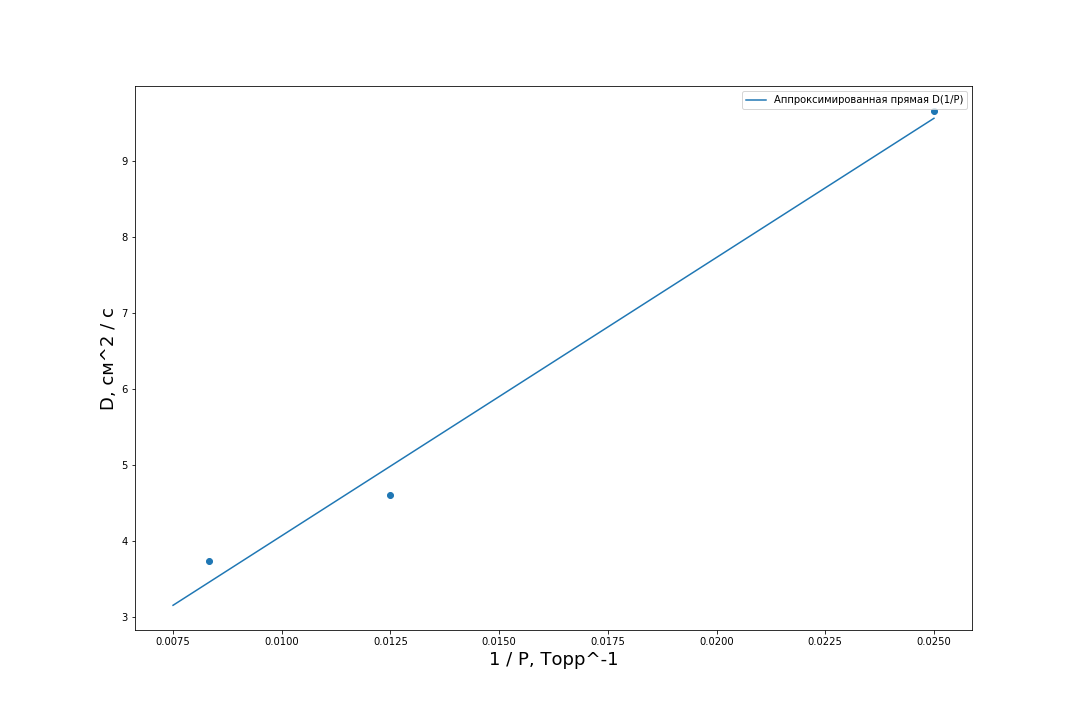
\includegraphics[width=\linewidth]{D_from_one_over_p_graph.png}
	\caption{График зависимости D(1/P)}
	\label{D_from_one_over_p_graph}
\end{figure}

\point Проведём аппроксимацию полученной зависимости прямыми $ y =kx + b $ методом линейной регрессии. В итоге получаем \[ k = (366.33 \pm 23.8) \text{ } \frac{\text{см}^2}{\text{с}\cdot\text{торр}}. \]

Таким образом, для атмосферного давления ($ P=760 $ торр) получаем \[{D_\text{атм} = (0.89\pm0.07) \text{ } \frac{\text{см}^2}{\text{с}}}, \quad (\varepsilon = 8\%). \]

\point По полученным ранее данным вычислим длину свободного пробега $ \lambda $ атомов гелия в воздухе. Согласно \eqref{2}:

\[ D = \frac{1}{3}\lambda \overline{v} = \frac{1}{3}\lambda\sqrt{\frac{8RT}{\pi\mu}}. \]

Отсюда получаем следующее:

\[{\lambda = 3D\sqrt{\dfrac{\pi\mu}{8RT}} \approx (105.74 \pm 7.1) \text{ нм}}, \quad (\varepsilon = 6.7\%).\]

\parag {Заключение} ~\\
В ходе работы:

\begin{enumerate}
	\item была зарегистрирована зависимость концентрации гелия в воздухе от времени при различных начальных давлениях смеси газов;
	\item по результатам измерений был определён коэффициент взаимной диффузии для смеси гелий-воздух;
	\item была оценена длина свободного пробега гения в воздухе.
\end{enumerate}

В итоге, для коэффициента взаимной диффузии смеси гелий-воздух мы получили:

\[{D_\text{атм} = (0.89\pm0.07) \text{ } \frac{\text{см}^2}{\text{с}}}, \quad (\varepsilon = 8\%). \]

Сравним полученные данные с табличными. Из таблицы в <<Лабораторном практикуме>> имеем:

\[ D_\text{табл} = 0.62 \text{ } \frac{\text{см}^2}{\text{с}}. \]

Таким образом, полученные экспериментально совпадают с табличными по порядку, что говорит об их достоверности, но отличаются от них даже с учетом погрешности. Отклонение от табличного значения могло возникнуть из-за неидеальных условий проведения эксперимента. Например, не всегда удавалось точно добиться необходимого начального давления, тем самым нарушалась балансировка моста и измерения могли исказиться.

Также была оценены длина свободного пробега гелия в воздухе:
\[{\lambda = 3D\sqrt{\dfrac{\pi\mu}{8RT}} \approx (105.74 \pm 7.1) \text{ нм}}, \quad (\varepsilon = 6.7\%).\]

Сравним полученные данные с табличными. Из справочников имеем:

\[ \lambda_\text{табл} = 175 \text{ нм}, \]

Видно, что полученный результат совпадает с табличным по порядку величины.

На мой взгляд, в основную погрешность в результаты эксперимента внесло некоторое несовпадение рассчитываемого рабочего давления с тем, что получается после наполнения экспериментальных сосудов газами. Такое различие вызывает разбаланc моста, что вносит определенную погрешность в измеряемые величины. Решить данную проблему можно, если дать более точные рекомендации по наполнению установки до рабочего давления.

\end{document}
